\documentclass{ximera}

\author{Anna Davis} \title{MTH 160 Homework 5} 

\begin{document}

\begin{abstract}

\end{abstract}
\maketitle
 \textit{Certificate due: 10/6/2021 at 11:59 p.m.}
 \section{Lecture 10}
 
  \begin{problem}\label{prob:160hom5prob1} 
  Solve the quadratic equation.  List your answers in an increasing order.
  \begin{enumerate}
      \item $$x^2-3x-4=0$$
      $$x=\answer{-1},\quad x=\answer{4}$$
      \item $$-3x^2+3x+8=0$$ (Round your answers to the nearest tenth.)
      $$x=\answer{-1.2},\quad x=\answer{2.2}$$
  \end{enumerate}
  \end{problem}
  
  \begin{problem}\label{prob:160hom5prob2} 
  Find the vertex.
  \begin{enumerate}
      \item $f(x)=-3x^2+3x+8$
      $$(\answer{0.5},\answer{8.75})$$
      \item $f(x)=x^2+2x+8$
      $$(\answer{-1},\answer{7})$$
  \end{enumerate}
  \end{problem}
  
  \begin{problem}\label{prob:160hom5prob3} 
  Find the equation of the line of symmetry for the parabola given by $f(x)=4x^2-16x+3$.
  $$x=\answer{2}$$
  \end{problem}
  
  \section{Lecture 11}
  
  \begin{problem}\label{prob:160hom5prob5} 
  Let $f(x)=(x+3)(x+1)(x-2)$.  
  
  List zeros of $f$ in an increasing order.
  $$x=\answer{-3},\quad x=\answer{-1},\quad x=\answer{2}$$
  
  The graph of $f$ is above the $x$-axis on the intervals
  $$(\answer{-3},\answer{-1})\quad \mbox{and}\quad (\answer{2},\answer{\infty})$$
  
  The graph of $f$ is below the $x$-axis on the intervals
  $$(\answer{-\infty},\answer{-3})\quad \mbox{and}\quad (\answer{-1},\answer{2})$$
  \end{problem}
  
  \begin{problem}\label{prob:160hom5prob6} 
  Sketch the graph of $f(x)=2x^4+2x^3-15x^2-10x+5$.
  \begin{center}  
\desmos{vnpejaj7ps}{800}{600}  
\end{center}
  Use the graph to find each of the following.  (Round your answers to three decimal places.)
  
  Zeros of $f$ (in increasing order).
  $$x=\answer{-2.892},\quad x=\answer{-1},\quad x=\answer{0.339},\quad x=\answer{2.554}$$
  
  Relative min (from left to right; rounded to three decimal places):
  $$y=\answer{-20.045} \mbox{ at } x=\answer{-2.198}$$
  $$y=\answer{-28.973}\mbox{ at } x=\answer{1.769}$$
  
  Relative max (rounded to three decimal places):
  $$y=\answer{6.619}\mbox{ at } x=\answer{-0.322}$$
    \end{problem}
    
\section{Lecture 12}   
\begin{problem}\label{prob:160hom5prob4} Use long-division to find the quotient.
\begin{enumerate}
  \item $$(x^3+3x^2-6x-8)\div (x-2)=\answer{x^2+5x+4}$$
  \item $$(x^3-3x^2-9x-5)\div (x-5)=\answer{x^2+2x+1}$$
  \end{enumerate}
  \end{problem}    
 
 \begin{problem}\label{prob:160hom5prob7}
 Find the $y$-intercept.
 $$f(x)=(x-1)(x+1)(x+10)(x-6)$$
 $$(0,\answer{60})$$
 \end{problem}
 
  \section{Lecture 13}
 
  \begin{problem}\label{prob:160hom6prob1} 
 A daycare center wishes to enclose a play area adjacent to the building, as shown in the diagram below.  If 200 linear feet of fencing is available, find the maximum possible area of the enclosure. 
 \begin{image}
   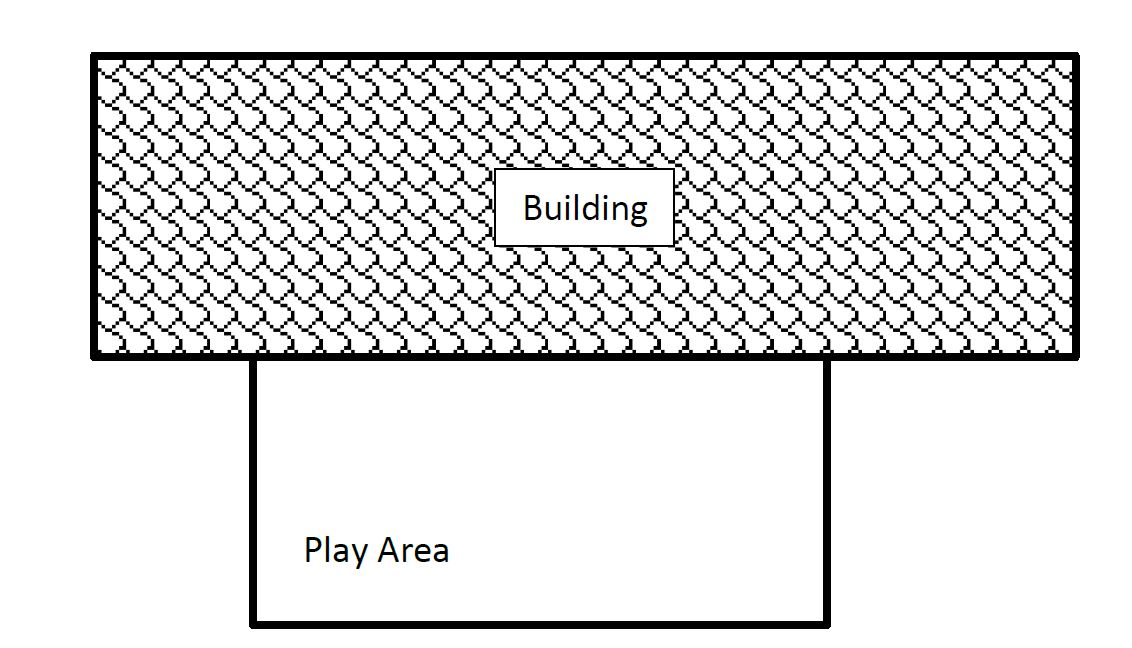
\includegraphics[height=1in]{160H6pic1.jpg}
 \end{image}
 Maximum possible area: $\answer{5000}$ sq. feet.
 \end{problem}
 \end{document}